

\documentclass[journal]{IEEEtran}

\usepackage[spanish,es-tabla]{babel}
\usepackage[utf8]{inputenc}

\hyphenation{op-tical net-works semi-conduc-tor}
\usepackage{algpseudocode}
\usepackage{graphicx} % Incluir figuras
\graphicspath{ {figuras/} }
\usepackage{amssymb}

\begin{document}

\title{Proyecto 1 - InstAA (Android App)}


\author{Josué Suárez Campos,~2016089518\\
       José Navarro Acuña,~2016254241 }
 
\markboth{Instituto Tecnológico de Costa Rica, Análisis de Algoritmos, Septiembre 2017}
{\MakeLowercase{\textit{et al.}}:}

\maketitle


\begin{abstract}
El presente artículo pretende exponer el funcionamiento, procedimiento análisis y experimentación de los algoritmos de filtrado. La aplicación permite el uso de tres tipos de filtrado: Blanco y negro, Gaussian Blur y un filtro propio. Además el filtro blanco y negro se divide en tres tipos, Averaging, Descomposition y Desaturation, los cuales se diferencian en su modo de crear el color gris. Se explicará, además, el algoritmo de convolución que permite a través de una matriz kernel, modificar la matriz de una imagen, método utilizado por el filtro Gaussian Blur y el filtro personalizado. Seguidamente, se hará el respectivo análisis de cada algoritmo con $O$ grande y así sacar su costo computacional. Para finalizar se expone una serie de experimentos con la aplicación que permitirá conocer su comportamiento a diferentes procesamientos.
\end{abstract}

\renewcommand{\IEEEkeywordsname}{Palabra clave}
\begin{IEEEkeywords}
Averaging, Convolution, Desaturation, Descomposition, Gaussian
\end{IEEEkeywords}



\IEEEpeerreviewmaketitle



\section{Introducción}

\IEEEPARstart{A}{}ctualmente las redes sociales son utilizadas por gran parte de la población mundial, plataformas como Facebook el cual cuenta con cerca de 1.900 millones de usuarios activos en un mes e Instagram que tiene más de 700 millones de usuarios activos. A estos sitios, además, son subidas millones de fotos a diario. Siguiendo el significado de la frase "\textit{Una imagen vale más que mil palabras}", gran parte de esta población intenta obtener un efecto llamativo en su fotografía, que exprese su sentir o forma de pensar. Es por ello que las plataformas que permiten la edición de imágenes son tan importantes actualmente, así como los diferentes filtros capaces de aplicar. La motivación de este proyecto radica en crear un programa que permita la aplicación de distintos filtros de manera rápida y eficaz utilizando el Procesamiento Digital de Imágenes (PDI) el cual es un conjunto de técnicas que se aplican a las imágenes digitales con el objetivo de mejorar la calidad o facilitar la búsqueda de información. Al ser una aplicación orientada a dispositivos móviles es importante recalcar que la aplicación es desarrollada para la plataforma Android, con la capacidad de ser ejecutada en dispositivos de este Sistema Operativo. 

 
\section{Conceptos Básicos}

A continuación se definen los conceptos básicos para esta investigación:\\
	\\
	\begin{itemize}
	\item{\bf Pixel:} Elemento primario de una imagen.
	\item{\bf Imagen:} Se refiere a una matriz bidimensional de píxeles con distinta propiedad luminosa.
	\item{\bf Color:} El color de una imagen es constituido por la mezcla de los colores primarios rojo, verde y azul (abreviados como RGB, en inglés). Los cuales se encuentran comúnmente en una escala de 0 a 255.
	\item{\bf Formato Gráfico:}  Son archivos en los cuales se guarda información que conforma una imagen.  Divididos en dos grupos: los formatos bitmap (mapa de bits) y los vectoriales. En el presente proyecto se utiliza el formato Bitmap.
	\item{\bf Algoritmo de Convolución:}  Serie de operaciones entre dos matrices lo cual permite cambiar el contenido de los pixeles de una imagen utilizando una matriz de tipo máscara. Este filtro máscara se nombrará en el artículo como Kernel. Más adelante se explicará con detalle su procedimiento.
	\end{itemize}

\section{Comportamiento Deseado}
La aplicación tiene dos funcionalidades para la selección de imágenes para posteriormente aplicar un filtro. La primera opcion corresponde al uso de la camara, siendo accesible en la pantalla principal, la segunda funcionalidad consiste en seleccionar una imagen de la galería del usuario, igualmente, es posible hacer uso de esta funcionalidad en la pantalla principal. Una vez seleccionada la imagen o fotografía, se despliegan mediante un panel horizontal, los filtros disponibles. \\

\begin{itemize}
	
	\item{\bf Blanco y negro}: Este filtro se divide en tres formas de aplicación. El primero de estos es el Averaging, el cual se logra con la suma de los colores RGB de un pixel donde posteriormente se dividen por 3. (Figura 1)
	
\end{itemize}	
	 % Figuras. Símbolos: h (here) - same location, t (top) - top of page, b (bottom) - bottom of page, p (page) - on an extra page, ! (override) - will force the specified location

	\begin{figure}[h]
		\centering
		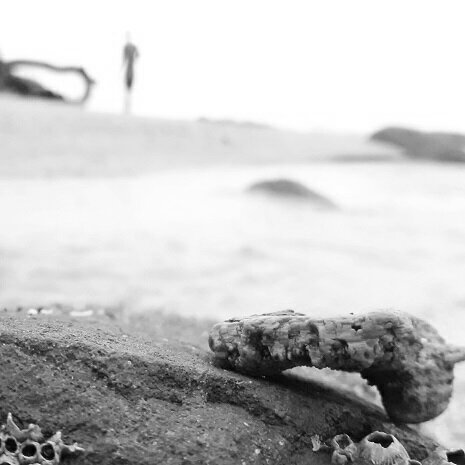
\includegraphics[width = 100pt]{averaging.jpeg}
		\caption{Averaging}
	\end{figure}

	La siguiente forma de este filtro es el Desaturation, cuyo proceso es la comparación entre los componentes RGB del pixel, del cual se extrae el elemento mayor y menor para luego ser sumados, por ultimo se aplica la división de ese valor por 2. (Figura 2) 
	
	\begin{figure}[h]
		\centering
		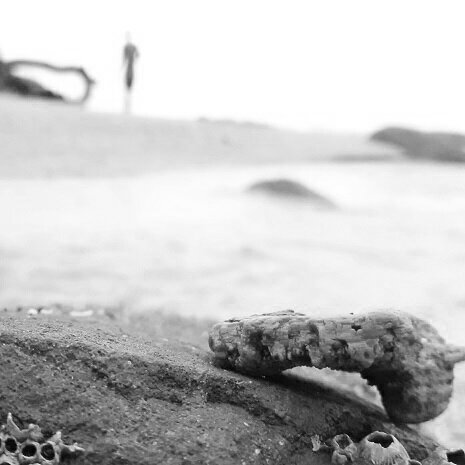
\includegraphics[width = 100pt]{desaturation.jpeg}
		\caption{Desaturation}
	\end{figure}
	
	\newpage
	Por último el filtro Decomposition, el cual se divide en dos, el Decomposition Min (Figura 3), cuyo valor gris se obtiene extrayendo el valor mínimo del RGB. El Decomposition Max (Figura 4), cuyo procedimiento es el opuesto al anterior, se extrae el valor minimo del componente RGB.
	
	\begin{figure}[h]
		\centering
		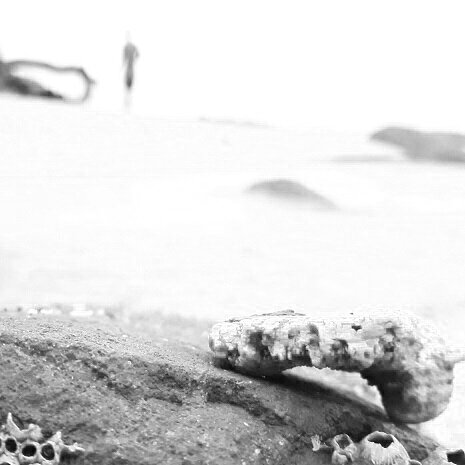
\includegraphics[width = 100pt]{desc-max.jpeg}
		\caption{Descomposition Max}
	\end{figure}


	\begin{figure}[h]
		\centering
		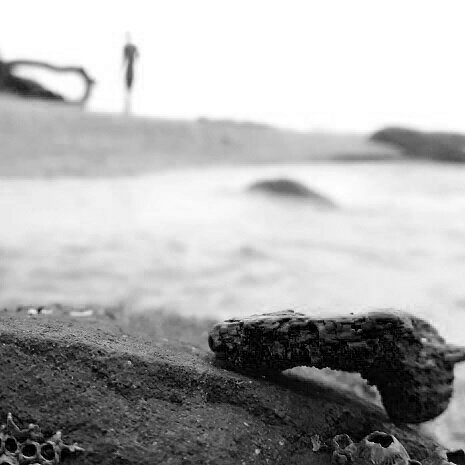
\includegraphics[width = 100pt]{desc-min.jpeg}
		\caption{Descomposition Min}
	\end{figure}

	
		
	
	\begin{itemize}
		\item{\bf Gaussian Blur:} Utiliza una matriz Gaussiana dinámica, la cual dependiendo de la entrada y el producto entre el largo por el ancho será construida, simulando entonces el comportamiento de la campana de Gauss. Con ello se logra un efecto borroso en la imagen (Figura 5).  Al seleccionar el filtro Gaussian Blur, aparecerá una barra selectora que permitirá personalizar la intensidad del efecto borroso en la imagen cuya escala de radio irá, de izquierda a derecha, menor a mayor (Figura 6). 
	\end{itemize}

	\begin{figure}[h]
		\centering
		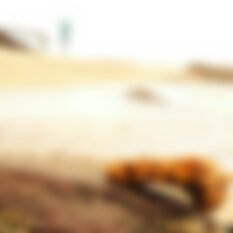
\includegraphics[width = 100pt]{gauss.jpeg}
		\caption{Gaussian}
	\end{figure}

	\begin{figure}[h]
		\centering
		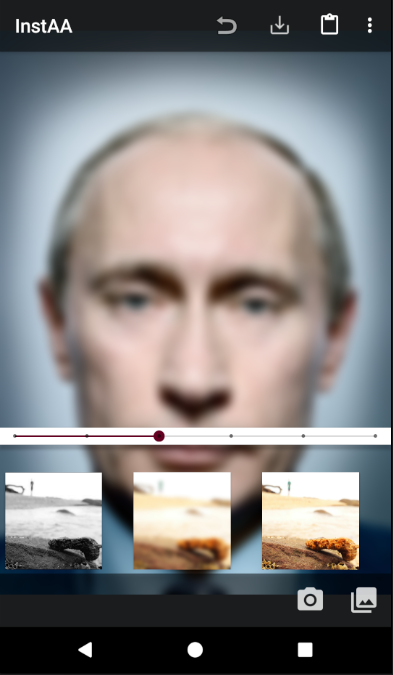
\includegraphics[width = 100pt]{personalizarBorrado.png}
		\caption{Personalizar intensidad del borrado}
	\end{figure}
		
	
	\newpage
	Este algoritmo utiliza el procedimiento de Convolución el cual consiste en colocar una matriz Kernel sobre la matriz de la imagen, los valores entrelazados se multiplican y se acumulan en variables, el resultado de esta acumulación es el valor RGB que toma la imagen filtrada. (Figura 7)
	
	\begin{figure}[h]
		\centering
		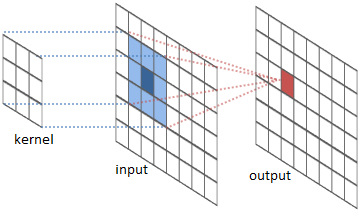
\includegraphics[width = 150pt]{convolution.png}
		\caption{Convolution}
	\end{figure}

	
	\begin{itemize}
		
	\item{\bf Filtro Personalizado:} Este filtro utiliza el algoritmo de convolución, realizando operaciones de multiplicación con una matriz (Ver Matriz 1). El valor del cada pixel está definido por defecto, es decir, el componente rojo contendrá un valor de 66, el verde un valor de 69, y el azul un valor de 99. Dichos valores se les restará el contenido del pixel original de la imagen, seguidamente se realiza la respectiva multiplicación con los valores del kernel. Los resultados se acumulan en variables las cuales corresponderán al valor del nuevo pixel. (Figura 8) \\
	
	\newpage
	La matriz kernel corresponde a la siguiente: \\
	Matriz 1
	\[ \left( \begin{array}{ccc} %Matriz 3x3
	-1 & 0 & 1 \\
	-2 & 0 & 2 \\
	-1 & 0 & 1 
	\end{array} \right)\]  \\
	
	Generando entonces, un comportamiento deseado como el siguiente:
	
	\end{itemize}

	\begin{figure}[h]
		\centering
		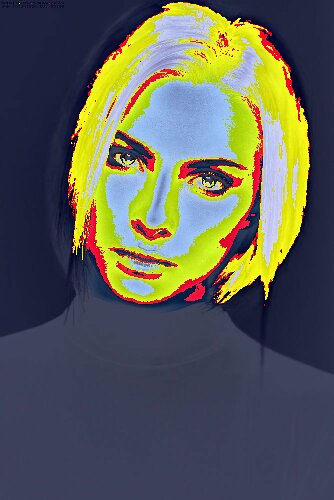
\includegraphics[width = 100pt]{filtrop.jpg}
		\caption{Filtro Personalizado}
	\end{figure}

	
	Si al seleccionar un filtro se desea volver a la imagen original basta con presionar el botón de Return, resaltado con círculo amarillo en la figura (Figura 9).
	\begin{figure}[h]
		\centering
		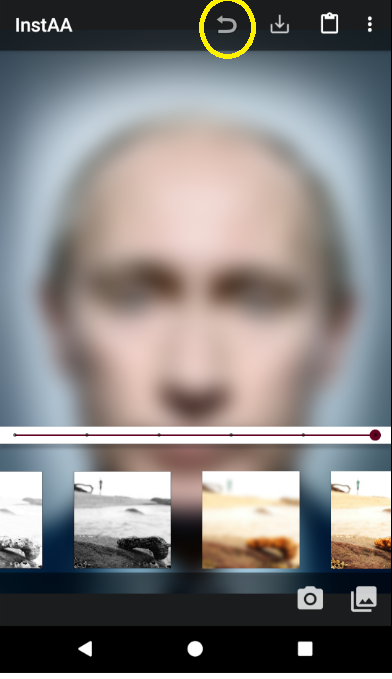
\includegraphics[width = 100pt]{return.png}
		\caption{Return}
	\end{figure}	

	Terminado de seleccionar el filtro para la imagen la aplicación permite guardarla en el dispositivo,  botón resaltado con círculo amarillo en la figura (Figura 10).
	
	\begin{figure}[h]
		\centering
		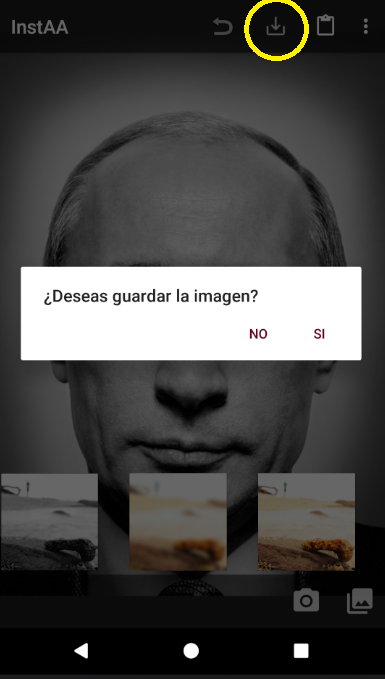
\includegraphics[width = 100pt]{guardar.png}
		\caption{Guardar Imagen}
	\end{figure}
	




\newpage
\section{Análisis}
En el siguiente apartado se hará el análisis de $O$ Grande de los algoritmos implementados.

	\begin{itemize}
		\item{\bf Blanco y negro:} Se muestra en las figuras 11 y 12 parte de la codificación del algoritmo blanco y negro. El cual inicia con un indice de valor 0 y se realizará hasta el valor de $ImageSize$, el cual es la multiplicación del alto y ancho de la imagen. Las demas operaciones que realizan los filtros (Averaging, Desaturation, entre otros.) son constantes, es decir, son operaciones elementales. Por tanto, se concluye que el costo del algoritmo es de $O(n \cdot m)$ donde $n$ es el ancho y $m$ el alto de la imagen entrada. Con respecto al barómetro, pertenece a la instrucción $for$ (Ver figura 12) donde hace posible iterar sobre el array de bits que contiene los pixeles de la imagen entrada y efectuar el filtro.
		
		
		
		\begin{figure}[h]
			\centering
			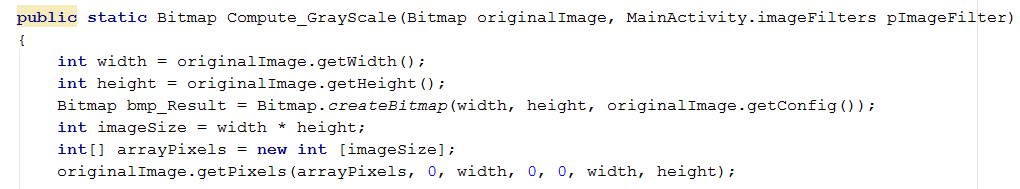
\includegraphics[height= 90pt, width=300pt]{bn1.png}
			\caption{Declaraciones}
		\end{figure}
	
	
	
		\begin{figure}[h]
			\centering
			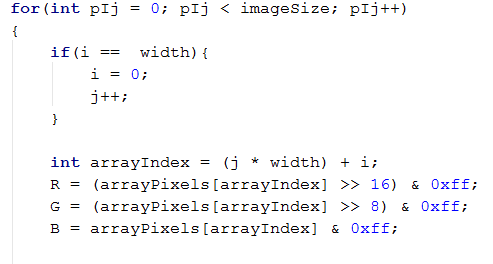
\includegraphics[height= 100pt, width=200pt]{bn2.png}
			\caption{Barómetro}
		\end{figure}
		
						
	\end{itemize}	

	
	

	\begin{itemize}
		\item{\bf Gaussian Blur:} Como se muestra en la figura 13 se hacen las declaraciones de la función, se obtiene el ancho y alto de la imagen además, se crea un nuevo bitmap reescalado en un 50\% de acuerdo a la imagen original, almacenando en un array los pixeles de la imagen original. Cabe mencionar, que dichas declaraciones son equivalentes a constantes, por tanto no afecta al orden.
		
		
		\begin{figure}[h]
			\centering
			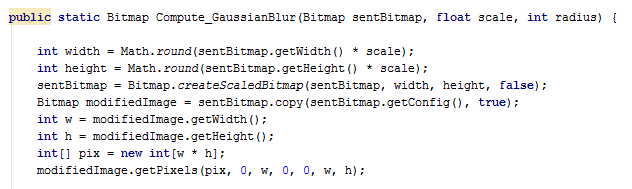
\includegraphics[height= 100pt, width=300pt]{1.png}
			\caption{Declaraciones}
		\end{figure}		
		
		En la figura 14 se puede apreciar dos ciclos $for$ anidados, donde el costo del primer $for$ es de $O(n)$ y el segundo $for$ es de $O(r)$, donde $n$ es el alto de la imagen y $r$ representa el radio (intensidad del efecto blur). Nuevamente, el cálculo que se realiza en $Math.min()$, además de los accesos al array $pix$ y $stack$, y las conversiones de bits a valores enteros; son constantes.
	
		\begin{figure}[h]
			\centering
			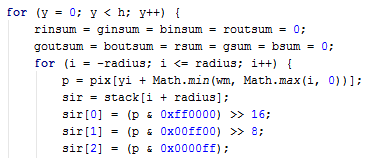
\includegraphics[height= 100pt, width=250pt]{3.png}
			\caption{Anidación de For}
		\end{figure}
	
		Seguidamente, en la figura 15 muestra un ciclo $for$ aninado al $for$ padre, este $for$ anidado tiene como coste $O(m)$, donde $m$ es el ancho de la imagen. Además no se encuentra anidado al ciclo $for$ con coste $O(r)$.
		Por lo tanto podemos concluir que el coste total de los tres ciclos $for$ es de $O(n \cdot (r + m))$. 
	
		\begin{figure}[h]
			\centering
			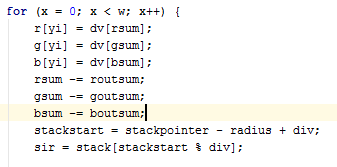
\includegraphics[height= 100pt, width=250pt]{4.png}
			\caption{For anidado al For 1}
		\end{figure}
		
		\newpage
		Continuando con el algoritmo Gaussiano, se muestra una nueva anidación de ciclos $for$ (Figura 16). El $for$ padre tiene como costo $O(m)$ y su anidado tiene un coste de $O(r)$ que igualmente, $m$ es el ancho de la imagen y $r$ representa el radio de la intensidad. Se presentan operaciones elementales de la cuales son ignoradas.
		
		\begin{figure}[h]
			\centering
			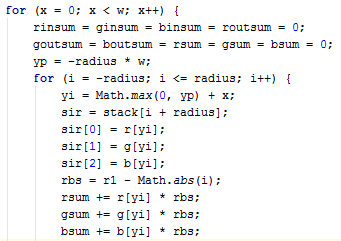
\includegraphics[height= 100pt, width=180pt]{5.png}
			\caption{Anidación de For}
		\end{figure}
	
		En la figura 17 se observa otro ciclo $for$ hijo, este se ejecuta $n$ veces porque depende del alto de la imagen entrada, por lo que su coste es de $O(n)$. Debido a las premisas anteriores el coste total de esta sección es de $O(m \cdot (n + r))$.
	
		\begin{figure}[h]
			\centering
			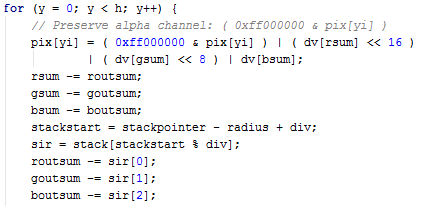
\includegraphics[height= 120pt, width=250pt]{6.png}
			\caption{Anidación de For}
		\end{figure}
	
		En consecuencia, se puede concluir que el coste total del algoritmo Gaussian Blur es $O(n \cdot (r + m) + m \cdot (n + r))$, ya que el primer $for$ tuvo un costo de $O(n \cdot (r + m))$, y el segundo de $O(m \cdot (n + r))$. \\
		Resolviendo la matemática para $f(n)$, se obtiene: \\
		
		\begin{center}
			$ f(n) = n \cdot (r + m) + m \cdot (n + r) $ \\
			$ = n \cdot r + n \cdot m + m \cdot r + m \cdot n $ \\
			$ = n \cdot r + m \cdot r + 2 \cdot n \cdot m $ \\
			$ = r(n + m) +n \cdot m $ \\
		\end{center}
	
	$\therefore O(r(n + m) +n \cdot m) $ \\
	
	En cuanto el barómetro, se consideraron los ciclos $for$ de la figura 14 y 16 para determinar el órden del algoritmo, por tanto, se considera que el barómetro se encuentra en los dos $for$ anteriormente mencionados, ya que hacen posible iterar sobre el arreglo de bits de la imagen, además de realizar el proceso de convolución creando un kernel dinámico.
	
	\end{itemize}

\newpage
	\begin{itemize}
		
		\item{\bf Filtro personalizado:} En la figura 18 se muestran las declaraciones más importantes del código del Filtro personalizado. En primer lugar, se efectúa el reescalamiento del tamaño de la imagen entrada en un 50\%, esto para optimizar el tiempo real de la ejecución del algoritmo. Seguidamente, se obtienen las dimensiones de la imagen reescalada para crear el arreglo de pixeles. Todo lo anterior mencionado tiene como órden constante, motivo por el cual es ignorado para determinar el órden del algoritmo.
	
		
		\begin{figure}[h]
			\centering
			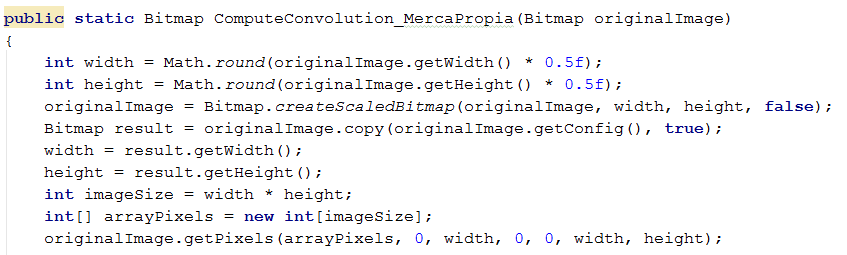
\includegraphics[height= 100pt, width=300pt]{mp1.png}
			\caption{Declaraciones}
		\end{figure}
	
		En la figura 19 se muestra el barómetro del código. El cual cada ciclo $for$ inicia con un indice de valor 0, el primer ciclo $for$ se realizará hasta el valor de $ImageSize$ el cual es la multiplicación del alto y ancho de la imagen, por lo que el costo sería de $O(n \cdot m)$ donde $n$ es el ancho y $m$ el alto. \\ 
		El segundo ciclo y tercer ciclo anidados, se repetirán hasta que el indice iguale el valor del tamaño del kernel, debido a esto el costo es $O(p^2)$. Por las declaraciones anteriores se puede concluir que el costo total del algoritmo es de $O(n \cdot m \cdot p^2)$.
	
		\begin{figure}[h]
			\centering
			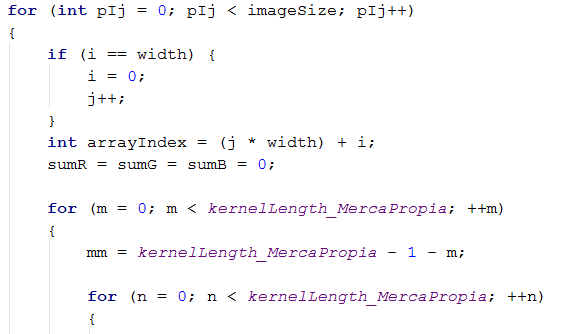
\includegraphics[height= 120pt, width=220pt]{mp2.png}
			\caption{Barómetro}
		\end{figure}
	
	
	\end{itemize}
	
		


\newpage
\section{Experimentos}
A continuación se exponen una serie de experimentos con la aplicación InstAA para conocer su comportamiento a diferentes situaciones. Cabe recalcar que estas comparaciones son efectuadas con un dispositivo Samsung J7-Prime con 3GB RAM y Procesador Exynos 7870 Octa octa-core 1.6 GHz, GPU Mali-T830MP2. Por tanto, los resultados obtenidos pueden variar dependiendo del dispositivo movil. \\
\begin{itemize}
	\item{\bf Comparación de duración en segundos:}  \\
	El primer experimento a efectuar consiste en calcular en segundos (s) la duración de cada algoritmo dependiendo del tamaño de la entrada. Para ello se utilizarán imágenes de tamaño 50x50, 100x100, 250x250, 465x465, 1000x1000 y finalmente 2000x2000. \\
	Primeramente, analizamos la gráfica del filtro Averaging dependiendo del tamaño de la imagen. Como se puede apreciar en la figura 20, el algoritmo aumenta su duración según van aumentado las dimensiones de la imágenes, donde una imagen menor a 1000x1000 apenas duraría 1 segundo de procesamiento, sin embargo una imagen 2000x2000 se procesa hasta cinco veces más que una menor a 1000x1000. 

	\begin{figure}[h]
		\centering
		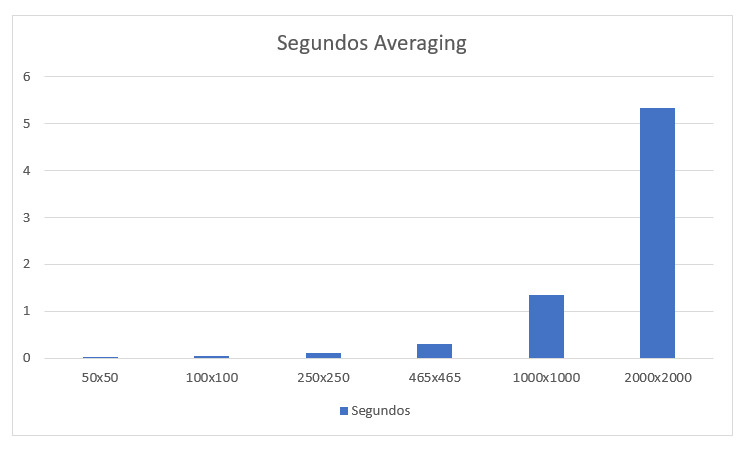
\includegraphics[height= 200pt, width=260pt]{msa.png}
		\caption{Averaging}
	\end{figure}


	Para el algoritmo de Desaturation (Figura 21) podemos observar que la duración de su procedimiento es baja para las imágenes con dimensiones menores a 1000x1000. Con una imagen 1000x1000 la duración de este algoritmo sería de 5 segundos y para una de 2000x2000 sería el cuádruple de la imagen anterior. Haciendo la comparación entre una imagen 2000x2000 de Averaging con Desaturation podemos observar que el algoritmo de Desaturation conlleva tres veces más tiempo. Por lo anterior podemos concluir el algoritmo de Desaturation conlleva mayor procesamiento que Averaging.
	
\newpage
	\begin{figure}[h]
		\centering
		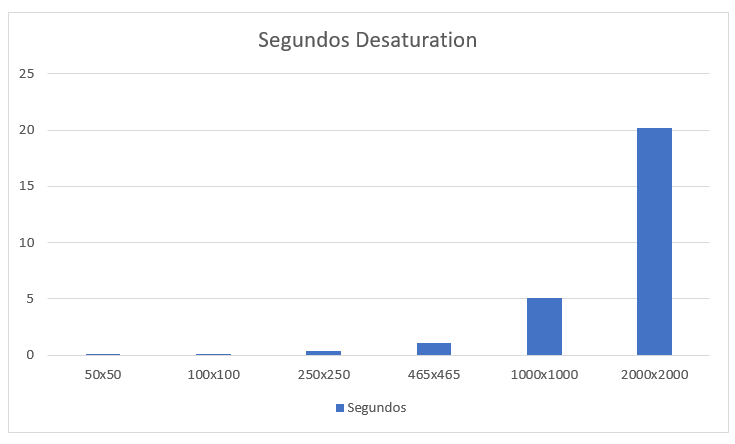
\includegraphics[height= 200pt, width=260pt]{msd.png}
		\caption{Desaturation}
	\end{figure}

	Analizando la gráfica de Descomposition Max se puede apreciar que, similar al filtro antecesor, su duración es muy baja para imágenes menores a 1000x1000 y a partir de esta dimensión su duración asciende a hasta los 17 segundos con una imagen 2000x2000. Podemos observar además que este filtro es de menor duración que el filtro Desaturation. 

	\begin{figure}[h]
		\centering
		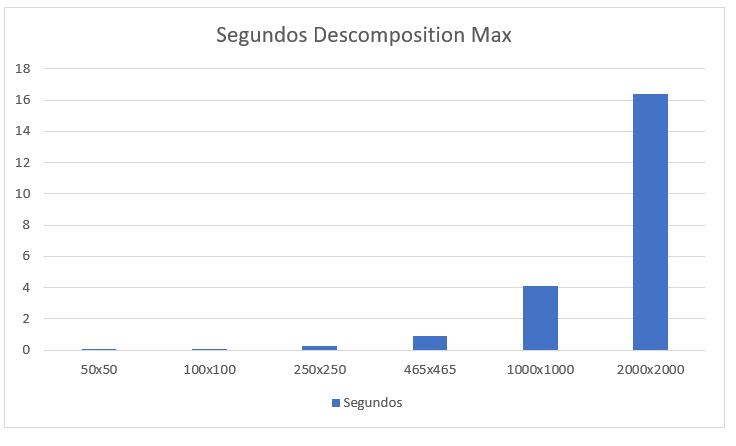
\includegraphics[height= 200pt, width=260pt]{msdm.png}
		\caption{Descomposition Max}
	\end{figure}

	En la figura 23 observamos el Descomposition Min con el mismo comportamiento que sus antecesores. Además notamos que tiene una ligera duración mayor al Descomposition Max llegando hasta 19 segundos con una imagen 2000x2000. 
\newpage
	\begin{figure}[h]
		\centering
		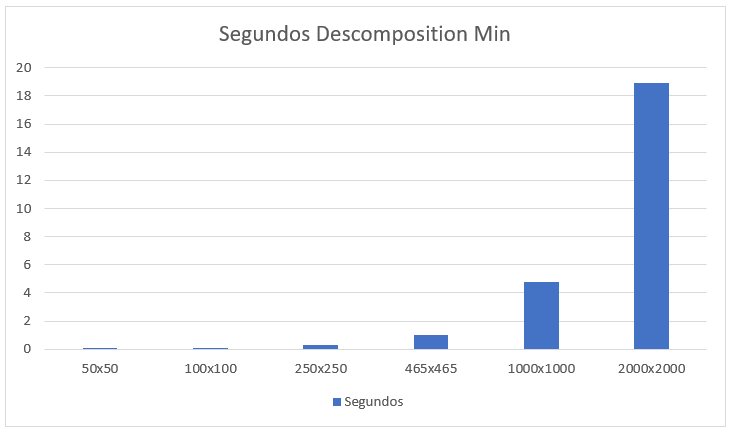
\includegraphics[height= 200pt, width=260pt]{msdmin.png}
		\caption{Descomposition Min}
	\end{figure}

	Para el filtro Gaussiano (figura 24) se puede apreciar la rapidez de este algoritmo con todas las dimensiones de imágenes, siendo la duración mayor la imagen de 2000x2000 con 4.5 segundos, aproximadamente la duración de los algoritmos anteriores con una imagen de 1000x1000 es la tercera parte de una 2000x2000.  

	\begin{figure}[h]
		\centering
		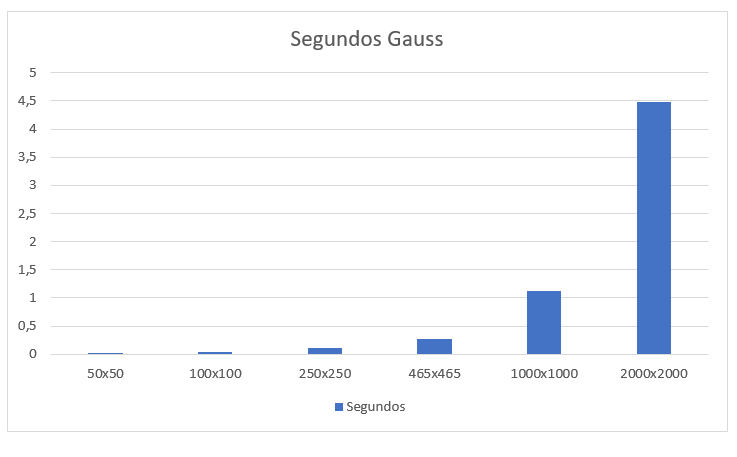
\includegraphics[height= 200pt, width=260pt]{msgauss.png}
		\caption{Gaussian}
	\end{figure}

	Con respecto al algoritmo del filtro personalizado (figura 25), se puede apreciar que para el proceso de una imagen de tamaño 100x100 el tiempo en milisegundos practicamente se duplica con respecto al procesamiento de una imagen de tamaño 50x50, siendo el tiempo real de un aproximado de 0.064 milisegundos. En comparación con una imagen de tamaño 250x250, el tiempo real supera por mucho más que el doble que el procesamiento del tamaño anterior, siendo éste de 0.294 milisegundos.

	\newpage
	\begin{figure}[h]
		\centering
		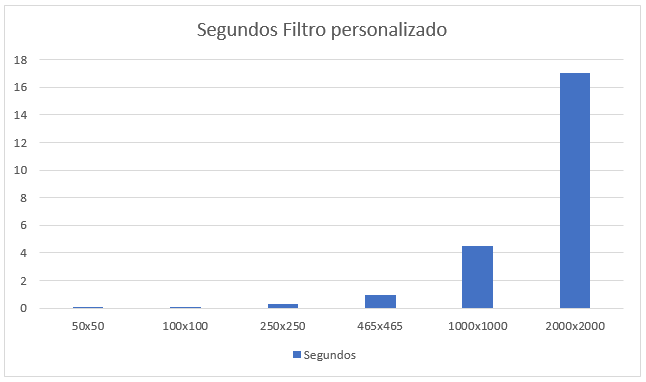
\includegraphics[height= 200pt, width=260pt]{msfp.png}
		\caption{Filtro personalizado}
	\end{figure}
	
	En conclusión, la siguiente grafica muestra el promedio de cada filtro segun su duración en tiempo real, es decir, una síntesis de las figuras anteriores.
	
	\begin{figure}[h]
		\centering
		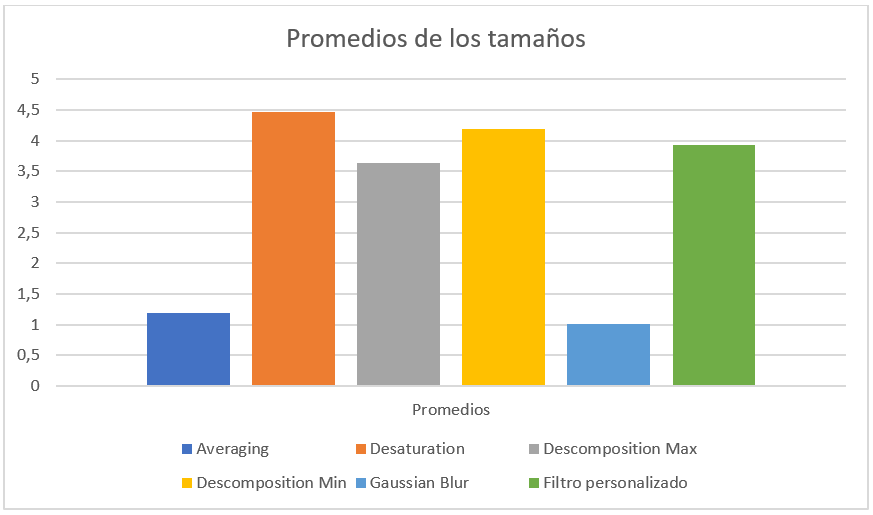
\includegraphics[height= 200pt, width=260pt]{promediosTiempo.png}
		\caption{Filtro personalizado}
	\end{figure}
	
	El filtro cuyo tiempo real supera a todos los demás, corresponde al Desaturation, con un plazo aproximado de 4.470 segundos en ejecución. El filtro de menor demanda corresponde al Gaussian Blur, donde su tiempo real equivale a 1.006 segundos. De forma comparativa, el filtro Desaturation hace uso exclusivamente de una función para obtener el valor del pixel en escala de gris, cuya funcionalidad, como se explicó anteriormente, es realizar dos operaciónes elementales; la suma entre el valor máximo y mínimo del RGB dividido entre 2. Por otro lado, el filtro Gaussian Blur, tomando en cuenta el proceso de convolución implementado y la calculación del kernel según las dimensiones de la imagen, se realiza el proceso de disminuir el tamaño de la imagen en un 50\% con respecto al tamaño original, sumado a ésto, el trabajar la altura y ancho por separado, además de manipular los pixeles con un array de bits, se obtuvo que el Gaussian Blur tiene la mejor eficiencia en cuanto al tiempo real. \\ 


	\item{\bf Comparación según rendimiento de CPU:} \\
	A continuación se hará una comparación de uso de CPU de todos los filtros dependiendo de la dimensión de entrada. \\
	Para imágenes 10x10 podemos observar que el uso del CPU es mínimo e insignificante ya que no llega ni al 10\% de la capacidad del dispositivo.

	De forma similar, el uso del CPU en imágenes 100x100 y 250x250 llegan a tener un pico máximo de 10\%, por tanto se utilizan pocos recursos. Sin embargo, el procesamiento requerido para una imagen 250x250 alcanza aproximadamente un 25\% de uso de la capacidad del dispositivo. En cuanto a las resoluciones de 465x465 y 1000x1000 se observa un cambio un tanto significativo de forma no prolongada formando una especie de montaña.

	\begin{figure}[h]
		\centering
		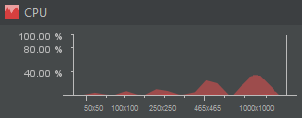
\includegraphics[height= 100pt, width=260pt]{rendimiento2.png}
		\caption{Promedio general del uso del CPU}
	\end{figure}

	A este punto, el panorama de rendimiento general para resoluciones de 2000x2000 pixeles es significante pero a la vez, se puede observar como el dispositivo limita de cierta manera los recursos del dispositivo movil, de tal forma que el tope maximo a utilizar es de un 40\% de una forma prologanda y no constante, ya que conforme aumenta el tiempo real en aplicar un filtro, la gráfica en un punto especifico se mantiene en forma de linea recta sin sobrepasar el limite establecido.

	\begin{figure}[h!]
		\centering
		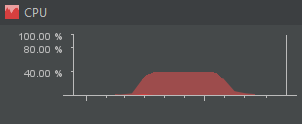
\includegraphics[height= 100pt, width=260pt]{2000x2000.png}
		\caption{Promedio del CPU para imágenes 2000x2000}
	\end{figure}

\newpage
	\item{\bf Comparación del tiempo real, de una imagen rectangular con una cuadrada:} \\
	El siguiente experimento a tratar, consiste en comparar el tiempo promedio de todos los filtros por haber, aplicados a una imagen rectangular, cuya resolución es de 2046 pixeles de ancho y 1100 de largo, por otro lado, la imagen cuadrada presenta una resolución de 1500 pixeles de ancho por 1500 pixeles de alto. \\
	Para iniciar, la imagen de tamaño rectangular presenta un total de 2.250.600 pixeles, y la imagen de tamaño cuadrado tiene un total de 2.250.000 pixeles. Como es evidente, se puede observar que la diferencia del total de pixeles de ambas imagenes es de solo 400 pixeles. Seguidamente, se medió el tiempo real de procesamiento de cada imagen el cual se hizo un promedio entre todos los filtros, tales resultados se aprecian en la figura 29.
	
	\begin{figure}[h!]
		\centering
		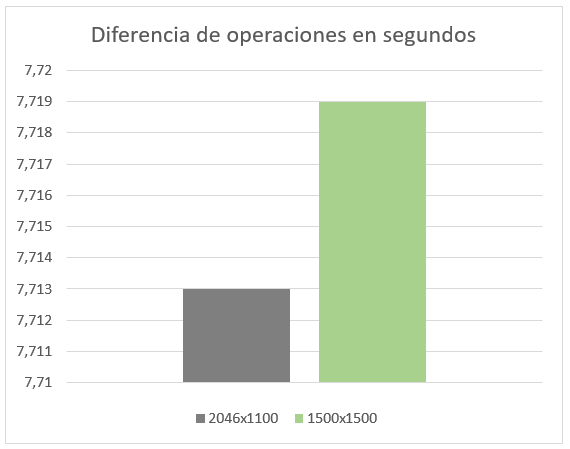
\includegraphics[height= 150pt, width=200pt]{DiferenciaOperaciones.png}
		\caption{Comparación del tiempo real según operaciones elementales}
	\end{figure}

	Podemos concluir que la duracion del procesamiento de una imagen cuadrada es mayor en décimas de segundo, exactamente 0.007 décimas, solo por una diferencia de 400 pixeles. Por lo tanto, dicho tamaño de imagen conlleva una mayor pero insignificante costo de procesamiento en comparación con la imagen rectangular.
	

\end{itemize}

\newpage
\section{Conclusión}

 En este proyecto se aprendió a elaborar, en el lenguaje de programación Java junto con la plataforma Android Studio, una aplicación para dispositivos móviles con Sistema Operativo Android. Se estudió el campo de la computación del procesamiento digital de imágenes y las técnicas de edición de estas mediante el uso de algoritmos y matrices numéricas. Comprendimos la estructura que conlleva una imagen digital y su representación en matrices matemáticas, además la composición de colores primarios digitales con su respectivo rango numérico (0-255). \\
Se instruyó en la elaboración de algoritmos para la aplicación de diferentes filtros a imágenes digitales tales como Averaging, Descomposition, Desaturation y Gaussian Blur. Se aplicó además un filtro personalizado mediante la experimentación con valores y operaciones matemáticas en el algoritmo de Convolución. Asimismo se realizaron experimentos para evaluar el funcionamiento y tiempo de ejecución de los algoritmos a distintas situaciones, tales como imágenes de distinto tamaño como entrada de la función y la evaluación del uso de recursos en el procesamiento de las imágenes. \\
Acerca de estos filtros se expuso que Desaturation es el de mayor duración y por el contrario el filtro Gaussian Blur el de menor duración de ejecución. Además en el uso del CPU se observó que el uso de este va aumentando según es mayor el tamaño de la imagen, sin embargo ninguno de los filtros junto con el tamaño de la imagen sobrepasan el 40\% del CPU.

\end{document}


